\chapter{Forschungsfragen}
\label{kap:forschungsfragen}
Hauptfokuspunkt der Masterarbeit sind Grafstrukturen in Form von Zugverkehrsnetzwerken. Eine Grafstruktur (siehe Abbildung \ref{fig_graph_structure}) besteht aus zwei Elementen, Knoten (Vertices) und Kanten (Edges). 
\begin{figure}[H]
    \caption{Beispiel einer Grafstruktur \parencite[S. 8]{wilson_2010}}
    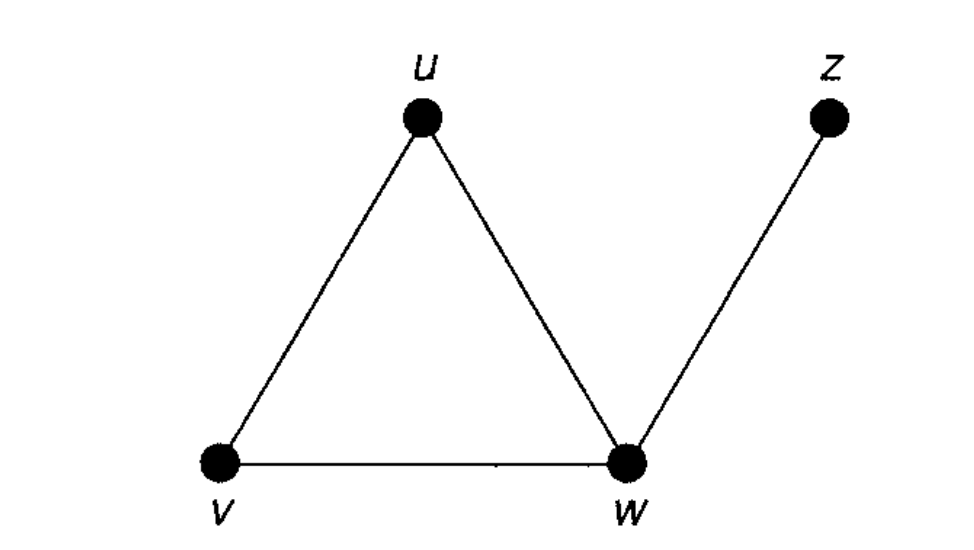
\includegraphics[width=.5\linewidth]{content/00_assets/graph_structure.png}
    \label{fig_graph_structure}
\end{figure}

Im Falle eines Zugnetzwerkes können die Knoten die einzelnen Stationen und die Kanten die Zuglinien widerspiegeln.  Es wird insbesondere das Zugverkehrsnetzwerk der \acrshort{sbb} betrachtet. Primär werden die Auswirkungen von Verspätungen auf ein solches Netzwerk analysiert. Die Hauptforschungsfrage der Arbeit lautet: 

\begin{itemize}
    \item \textbf{Welche Trends und Anomalien ergeben sich im dynamischen Zugnetzwerk der SBB?}
\end{itemize}

Abgeleitet von dieser Hauptforschungsfrage ergeben sich folgende interessante untergeordnete Fragen:

\begin{itemize}
    \item \textbf{Welche Zugstationen und Zuglinien sind am stärksten von Verspätungen betroffen und welche Clusterbildungen entstehen hieraus?}
    \item \textbf{Welche zeitlichen Muster ergeben sich pro Zuglinie und Station in Hinblick auf Verspätungen?}
\end{itemize}
